% Provenance (never printed): sources/book2/BRIEFS.md, g11-06. Private and social cost, the deadweight loss of an
% externality, the Coase result, the Pigouvian tax, tradable permits and standards, positive externalities, and
% government failure. Real numbers: figdata/grade-11/06-externalities/ (CEDS SO2 and Maddison, 1850-2022; CEDS US
% SO2 1970-2023; the Acid Rain Program dates as a cited table). Ledger: Schmalensee and Stavins 2013, EPA Acid Rain
% Program, Andersson 2019, Farnsworth 1999 and Abildtrup et al. 2012 (via a reference page). No published estimate of
% the cost saving of SO2 trading was read, so none is printed. Photograph: the 1952 London smog (Commons, CC BY-SA 2.0). The tannery
% and the fishery are invented.
\chapter{Externalities}\label{ch:g11:externalities}

In 1918 the United States emitted about 191 kilograms of sulphur dioxide for each of its inhabitants, mostly from burning coal. Britain had
peaked a decade earlier, at 134 kilograms. By 2022 the American figure was 5.1 kilograms and the British 1.7, while incomes per person had grown
several times over. China's emissions per person peaked in 2006 at 29 kilograms and fell to 7.5 by 2022. Sulphur dioxide makes acid rain and fills
lungs with fine particles; it harms people who neither produced nor bought the electricity whose making released it.
% figdata: so2_peaks (USA 1918 190.78 -> 5.07; GBR 1907 133.98 -> 1.72; CHN 2006 29.00 -> 7.45)

Such harm is a cost that no price records. This chapter shows why a market then produces too much of the harmful good, and compares the ways of
correcting it: bargaining, taxes, \omterm{def:g11:externalities:tradable-permit}{tradable permits} and rules, each with its evidence. The fall in the chart came with laws, and with changes in
fuels and technology; the second chart of the chapter shows one of those laws at work, and what it can and cannot tell.

\begin{openingchart}{Sulphur dioxide emissions per person against GDP per person, six countries, 1850--2022, both on times-ten scales; one point every five years.
Emissions in kilograms a year; GDP per person in 2011 dollars at purchasing-power parity.}{Community Emissions Data System (CEDS), sulphur dioxide by country;
Maddison Project Database 2023, GDP per person and population}
\begin{tikzpicture}
\begin{loglogaxis}[omscatter, log basis x=10, log basis y=10, log ticks with fixed point, width=0.86\linewidth, height=7.0cm,
  xmin=400, xmax=100000, ymin=0.05, ymax=300, xtick={1000,10000,100000}, ytick={0.1,1,10,100},
  xlabel={GDP per person (dollars a year)}, ylabel={SO$_2$ per person (kg a year)}]
\addplot[omThm, thick, sharp plot, mark=*, mark size=0.7pt] table[x=gdppc, y=so2pc] {figdata/grade-11/06-externalities/out/so2_USA.csv}
  node[pos=1, right, font=\scriptsize] {USA};
\addplot[omDef, thick, sharp plot, mark=*, mark size=0.7pt] table[x=gdppc, y=so2pc] {figdata/grade-11/06-externalities/out/so2_GBR.csv}
  node[pos=1, anchor=north east, font=\scriptsize] {GBR};
\addplot[omProp, thick, sharp plot, mark=*, mark size=0.7pt] table[x=gdppc, y=so2pc] {figdata/grade-11/06-externalities/out/so2_DEU.csv}
  node[pos=1, anchor=north west, font=\scriptsize] {DEU};
\addplot[omMeth, thick, sharp plot, mark=*, mark size=0.7pt] table[x=gdppc, y=so2pc] {figdata/grade-11/06-externalities/out/so2_JPN.csv}
  node[pos=1, anchor=south east, font=\scriptsize] {JPN};
\addplot[omExo, thick, sharp plot, mark=*, mark size=0.7pt] table[x=gdppc, y=so2pc] {figdata/grade-11/06-externalities/out/so2_CHN.csv}
  node[pos=1, above, font=\scriptsize] {CHN};
\addplot[black, thick, sharp plot, mark=*, mark size=0.7pt] table[x=gdppc, y=so2pc] {figdata/grade-11/06-externalities/out/so2_IND.csv}
  node[pos=1, right, font=\scriptsize] {IND};
\end{loglogaxis}
\end{tikzpicture}
\end{openingchart}

\begin{recall}
From the grades 6--9 volume: sulphur dioxide, released when coal and oil are burned, rose as countries
industrialised and later fell in the richest ones. From
\cref{ch:g10:surplus-and-efficiency}: \omterm{def:g10:surplus-and-efficiency:total-surplus}{total surplus}, and why the market quantity maximises it when prices carry all costs and benefits. From
\cref{ch:g10:tax-incidence}: a tax per unit and its incidence. The physics and chemistry of acid rain and of the climate are left to the Earth and space sciences
volumes; this chapter takes the damage as given.
\end{recall}

\section{Private cost and social cost}\label{sec:g11:externalities:social-cost}

\begin{definition}[Externality]\label{def:g11:externalities:externality}
An \emph{externality}\index{externality} is an effect of a person's or firm's activity on others that is not paid for through a price. It is a \emph{negative
externality}\index{negative externality}\phantomsection\label{def:g11:externalities:negative} when it harms them, a \emph{positive
externality}\index{positive externality}\phantomsection\label{def:g11:externalities:positive} when it benefits them.
\end{definition}

\begin{omfigure}
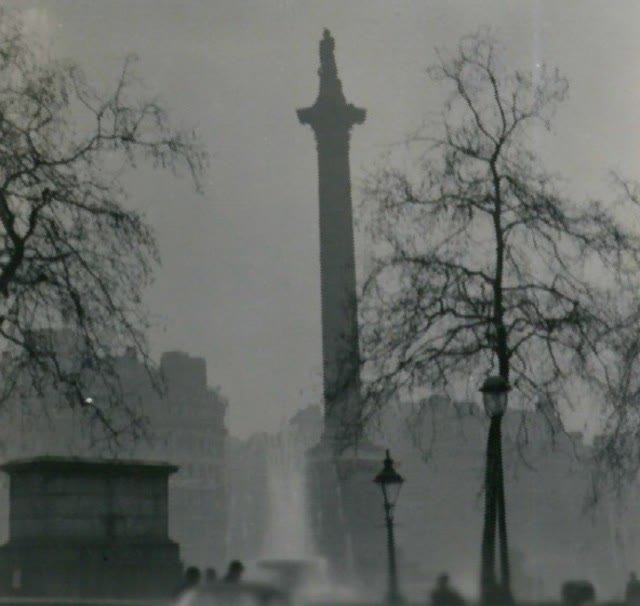
\includegraphics[width=0.58\linewidth]{images/book2/photos/g11-externalities-london-smog-1952.jpg}

{\small Nelson's Column in London during the smog of December 1952. The smoke of the coal burnt in homes and factories fell on everyone who breathed the air, and no price charged those who burnt it for that. Photograph: N T Stobbs, CC BY-SA 2.0.}
\end{omfigure}

\begin{definition}[Private, external and social cost]\label{def:g11:externalities:private-cost}
The \emph{private cost}\index{private cost} of a good is the cost borne by its producer. The \emph{external cost}\index{external cost}%
\phantomsection\label{def:g11:externalities:external-cost} is the cost it imposes on others. The \emph{social cost}\index{social cost}%
\phantomsection\label{def:g11:externalities:social-cost} is their sum. In the same way, the \emph{social benefit}\index{social benefit}%
\phantomsection\label{def:g11:externalities:social-benefit} of a good is the benefit to its buyers plus the benefit to others.
\end{definition}

\begin{example}[A polluting market]\label{ex:g11:externalities:market}
Demand for a good is $p = 100 - Q$, its private \omterm{def:g11:marginal-reasoning:marginal-benefit}{marginal cost} is $20 + Q$, and each unit causes damage of 20 dalens to people nearby. The market settles where demand
meets private \omterm{def:g11:marginal-reasoning:marginal-benefit}{marginal cost}: $Q = 40$, $p = 60$. The social \omterm{def:g11:marginal-reasoning:marginal-benefit}{marginal cost} is $40 + Q$, and it equals the buyers' \omterm{def:g11:marginal-reasoning:marginal-benefit}{marginal benefit} at $Q = 30$. The ten units between
30 and 40 cost society more than they are worth to buyers; the lost surplus is $\tfrac12 \times (40 - 30) \times 20 = 100$ dalens.
\end{example}

\begin{omfigure}
\begin{tikzpicture}[econ, x=0.085cm, y=0.055cm]
\draw[econ axes] (0,105) node[left, font=\small] {dalens} |- (80,0) node[below left=12pt and 0pt, font=\small] {$Q$};
\fill[omThm!25] (30,70) -- (40,80) -- (40,60) -- cycle;
\draw[demand] (0,100) -- (75,25) node[right, font=\scriptsize] {demand (marginal benefit)};
\draw[supply] (0,20) -- (65,85) node[right, font=\scriptsize] {private marginal cost};
\draw[omThm, thick] (0,40) -- (55,95) node[right, font=\scriptsize] {social marginal cost};
\node[eqpoint] at (40,60) {}; \node[eqpoint] at (30,70) {};
\draw[guide] (0,60) -- (40,60) -- (40,0); \draw[guide] (0,70) -- (30,70) -- (30,0); \draw[guide] (30,50) -- (0,50);
\draw[<->, thin] (44,60) -- (44,80); \node[font=\scriptsize, right] at (44.5,70) {20};
\foreach \y in {50,60,70} \draw (0,\y) -- (-1,\y) node[left, font=\footnotesize] {\y};
\node[below, font=\footnotesize] at (30,0) {30}; \node[below, font=\footnotesize] at (40,0) {40};
\end{tikzpicture}

{\small The market sells 40 units, where demand meets private \omterm{def:g11:marginal-reasoning:marginal-benefit}{marginal cost}; the efficient quantity is 30, where it meets social \omterm{def:g11:marginal-reasoning:marginal-benefit}{marginal cost}. The shaded triangle,
100 dalens, is the \omterm{def:g10:what-prices-do:dwl}{deadweight loss}. A tax of 20 a unit, the marginal damage, makes buyers pay 70 and sellers receive 50, and the market sells 30.}
\end{omfigure}

\section{Bargaining}\label{sec:g11:externalities:coase}

The damage is a conflict over the use of something, the air or a river, whose owner is not clear. If the right were clearly given to one side, the two could
bargain.

\begin{definition}[Transaction cost]\label{def:g11:externalities:transaction-cost}
A \emph{transaction cost}\index{transaction cost} is the cost of making a deal: finding the other parties, learning the facts, negotiating, writing the agreement
and enforcing it.
\end{definition}

\begin{proposition}[The Coase result]\label{prop:g11:externalities:coase}
\index{Coase theorem}Suppose a polluter gains $B(q)$ and a victim loses $D(q)$ from an activity $q$, the right to decide $q$ is clearly held by one of them, and they can
make any agreement at no \omterm{def:g11:externalities:transaction-cost}{transaction cost}, paying each other money. Then they agree on the $q$ that maximises $B(q) - D(q)$, whichever of them holds the right. The
right decides only who pays whom.
\end{proposition}
\begin{proof}
Any $q$ that does not maximise $B - D$ leaves a gain unclaimed: moving to the maximising $q^*$ raises $B - D$, and a payment from the side that gains to the side
that loses can share that rise so that both are better off. So a deal stops only at $q^*$. If the victim holds the right, the polluter pays to be allowed $q^*$; if
the polluter holds it, the victim pays it to cut back to $q^*$. Either way $q = q^*$.
\end{proof}

\begin{model}{The Coase result}
\assumes Rights are clear, the parties are few and know the costs and benefits, and bargaining is cheap.
\predicts An efficient outcome whoever holds the right; the right decides who pays.
\tested In twenty nuisance cases followed after a court had ruled, none of the parties tried to bargain, although the ruling made the rights clear: they were angry with
  each other (Farnsworth 1999). In negotiations between Danish waterworks and the farmers around their wells, farmers used what only they knew to ask for more than
  their losses, and some talks broke off (Abildtrup, Jensen and Dubgaard 2012).
\breaks When the parties are many (everyone who breathes a city's air), when costs are private information, and when bargaining itself is costly or resented.
\end{model}
% ledger: g11:farnsworth1999, g11:abildtrup2012

\section{Taxes, permits and rules}\label{sec:g11:externalities:instruments}

\begin{definition}[Pigouvian tax]\label{def:g11:externalities:pigouvian-tax}
A \emph{Pigouvian tax}\index{Pigouvian tax} is a tax on each unit of a harmful activity equal to its marginal \omterm{def:g11:externalities:private-cost}{external cost} at the efficient quantity.
\end{definition}

The tax puts the damage into the producer's own cost. In the example, a tax of 20 a unit shifts private \omterm{def:g11:marginal-reasoning:marginal-benefit}{marginal cost} onto social \omterm{def:g11:marginal-reasoning:marginal-benefit}{marginal cost}, and the market
itself sells the efficient 30 units. The government collects $20 \times 30 = 600$ dalens, which it can spend or return.

\begin{model}{The Pigouvian tax}
\assumes The marginal \omterm{def:g11:externalities:private-cost}{external cost} is known and the same for every unit wherever it is produced; producers respond to prices.
\predicts A tax equal to the marginal damage brings the market to the efficient quantity, and each producer cuts back where cutting is cheapest.
\tested After Sweden added a carbon tax, and a value-added tax, to the price of transport fuels, carbon dioxide emissions from transport were almost
  11\,\% lower than in a comparison built from similar countries without them, most of it due to the carbon tax (Andersson 2019).
\breaks When the damage is unknown, or differs from one place to another (a factory upwind of a city does more harm than one in a desert); when the rate is set by
  lobbying rather than by the damage.
\end{model}
% ledger: g11:andersson2019

\begin{definition}[Tradable permit]\label{def:g11:externalities:tradable-permit}
A \emph{tradable permit}\index{tradable permit} is a right to emit one unit of a pollutant, which its holder may use or sell. The authority sets the total number of
permits, the cap, and the permits trade at a market price.
\end{definition}

\begin{definition}[Emission standard]\label{def:g11:externalities:standard}
An \emph{emission standard}\index{emission standard} is a rule limiting how much each source may emit, or which technology it must use.
\end{definition}

A tax fixes the price of emitting and lets the quantity adjust; a permit market fixes the quantity and lets the price adjust. Both make every polluter cut back until
its cost of cutting one more unit equals the same price, so the total cut is made where it is cheapest. A uniform standard asks every source to cut the same amount,
whatever it costs them; it costs more for the same total cut, unless all sources have the same costs.

\begin{omfigure}
\begin{tikzpicture}[econ, x=0.13cm, y=0.06cm]
\begin{scope}
\draw[econ axes] (0,90) node[left, font=\small] {dalens a tonne} |- (44,0) node[below left=12pt and 0pt, font=\small] {tonnes cut};
\draw[supply] (0,0) -- (40,40) node[right, font=\scriptsize] {firm A};
\draw[demand] (0,0) -- (20,80) node[right, font=\scriptsize] {firm B};
\draw[omThm, thick] (0,32) -- (40,32) node[right, font=\scriptsize] {permit price 32};
\node[eqpoint] at (32,32) {}; \node[eqpoint] at (8,32) {};
\draw[guide] (32,32) -- (32,0); \draw[guide] (8,32) -- (8,0); \draw[guide] (20,80) -- (20,0);
\node[below, font=\footnotesize] at (8,0) {8}; \node[below, font=\footnotesize] at (20,0) {20}; \node[below, font=\footnotesize] at (32,0) {32};
\foreach \y in {20,32,80} \draw (0,\y) -- (-0.5,\y) node[left, font=\footnotesize] {\y};
\end{scope}
\end{tikzpicture}

{\small \omterm{def:g11:marginal-reasoning:marginal-benefit}{Marginal cost} of cutting emissions for two tanneries (the weekend problem): $x$ for A and $4x$ for B, with $x$ the tonnes cut. A standard of 20 tonnes each
costs B 80 dalens for its last tonne and A only 20. With permits for a total cut of 40, the permit price settles at 32: A cuts 32 tonnes and B 8.}
\end{omfigure}

\begin{model}{Tradable permits}
\assumes The authority can measure every source's emissions; firms buy and sell permits freely.
\predicts Emissions fall to the cap; the cuts are made by the sources that can cut most cheaply; the permit price reflects the cost of the last tonne cut.
\tested The American market for sulphur dioxide permits, created by the Clean Air Act Amendments of 1990, performed well, and a large part of its low cost came from
  a change it did not plan, the earlier deregulation of the railways (Schmalensee and Stavins 2013).
\breaks When emissions cannot be measured; when permits are given away to the firms with the best lobbyists; when courts or new rules undo the cap, as later happened to
  this market.
\end{model}
% ledger: g11:caa-1990

\begin{omchart}{Sulphur dioxide emissions of the United States, 1970--2023, in millions of tonnes a year. The lines mark the 1990 law and the starts of the two phases of
the Acid Rain Program, in 1995 and 2000.}{Community Emissions Data System (CEDS); dates: US Environmental Protection Agency}
\begin{tikzpicture}
\begin{axis}[omtime, width=0.84\linewidth, height=5.4cm, xmin=1970, xmax=2023, ymin=0, ymax=32, ylabel={million tonnes}, xtick={1970,1980,...,2020}]
\addplot[omDef, thick] table[x=year, y=mt] {figdata/grade-11/06-externalities/out/so2_usa.csv};
\addplot[black, dashed, ycomb, no markers] table[x=year, y=top] {figdata/grade-11/06-externalities/out/arp_dates.csv};
\end{axis}
\end{tikzpicture}
\end{omchart}
% ledger: g11:caa-1990, g11:arp-phases; figdata: so2_usa (1990 21.07, 2010 6.21, 2023 1.49)

\begin{record}[The US acid-rain programme, 1995--2010]
% ledger: g11:arp-phases, g11:caa-1990; figdata: so2_usa
The law of 1990 set a cap on the sulphur dioxide of American power plants and let them trade allowances. The first phase began in 1995 and the second in 2000; the final
cap, from 2010, was 8.95 million tons, about half the power sector's emissions of 1980. National emissions
of the gas, from all sources, fell from 21.07 million tonnes in 1990 to 6.21 million in 2010. The chart cannot say how much of the fall the programme caused: emissions
were already falling before 1990, under earlier rules.
\end{record}

\section{Positive externalities}\label{sec:g11:externalities:positive}

A person vaccinated against a contagious disease protects herself and, by not passing it on, others. A firm that discovers a new method teaches its rivals, who copy it.
In such cases the \omterm{def:g11:externalities:private-cost}{social benefit} is above the private benefit, and the market produces too little. The mirror of the \omterm{def:g11:externalities:pigouvian-tax}{Pigouvian tax} is a subsidy equal to the marginal
external benefit: it raises the quantity to where \omterm{def:g11:externalities:private-cost}{social benefit} equals cost. Research grants, patents, and free or compulsory vaccination are its forms.

\section{When the cure fails}\label{sec:g11:externalities:failure}

The instruments need numbers that governments must estimate, and governments can get them wrong. A tax set above the marginal damage cuts the activity too far, with a
\omterm{def:g10:what-prices-do:dwl}{deadweight loss} of its own. Permits handed out free to existing firms reward past polluters and can keep newcomers out. Exemptions are won by the industries that lobby
hardest. And a rule can be written in one year and undone in the next. \Cref{ch:g11:public-choice-first-look} studies how such choices are made.

\section{Exercises}

\begin{exercise}[$\star$]\label{exo:g11:externalities:1}
A factory's private \omterm{def:g11:marginal-reasoning:marginal-benefit}{marginal cost} of the 1st to 4th tonne of output is 10, 12, 14 and 16 dalens, and each tonne causes damage of 5 to its neighbours. Give the social
\omterm{def:g11:marginal-reasoning:marginal-benefit}{marginal cost} of each tonne.
\end{exercise}

\begin{exercise}[$\star$]\label{exo:g11:externalities:2}
The \omterm{def:g11:externalities:private-cost}{private cost} of a flight is 300 dalens and its emissions cause damage of 45 dalens. What is its \omterm{def:g11:externalities:private-cost}{social cost}? What share of it does the airline bear?
\end{exercise}

\begin{exercise}[$\star$]\label{exo:g11:externalities:3}
Read the opening chart. Which country emitted the most sulphur dioxide per person, and in which year? At about what income per person did the United States, Britain
and Japan reach their peaks?
\end{exercise}

\begin{exercise}[$\star$]\label{exo:g11:externalities:4}
Demand is $p = 80 - Q$, private \omterm{def:g11:marginal-reasoning:marginal-benefit}{marginal cost} is $Q$, and the marginal damage is 20 a unit. Find the market quantity and the efficient quantity.
\end{exercise}

\begin{exercise}[$\star$]\label{exo:g11:externalities:5}
In \cref{exo:g11:externalities:4}, what tax brings the market to the efficient quantity? What do buyers pay and sellers receive?
\end{exercise}

\begin{exercise}[$\star\star$]\label{exo:g11:externalities:6}
Compute the \omterm{def:g10:what-prices-do:dwl}{deadweight loss} of the \omterm{def:g11:externalities:externality}{externality} in \cref{exo:g11:externalities:4}.
\end{exercise}

\begin{exercise}[$\star\star$]\label{exo:g11:externalities:7}
Demand is $p = 130 - 2Q$, private \omterm{def:g11:marginal-reasoning:marginal-benefit}{marginal cost} $10 + Q$, and the marginal damage $Q$ (it grows with the quantity). Find the market and efficient quantities, the
\omterm{def:g11:externalities:pigouvian-tax}{Pigouvian tax} and the \omterm{def:g10:what-prices-do:dwl}{deadweight loss}.
\end{exercise}

\begin{exercise}[$\star\star$]\label{exo:g11:externalities:8}
A farmer's crops are damaged by a neighbour's goats. Keeping the goats is worth 300 dalens a year to the neighbour; the damage is 500. Fencing them in would cost 200.
What happens if the neighbour has the right to let the goats roam? If the farmer has the right to be free of them?
\end{exercise}

\begin{exercise}[$\star\star$]\label{exo:g11:externalities:9}
Same question if the damage is 150 a year.
\end{exercise}

\begin{exercise}[$\star\star$]\label{exo:g11:externalities:10}
In the tanneries' permit market of the figure, the cap is tightened so that the total cut must be 50 tonnes. Find the new permit price and each tannery's cut.
\end{exercise}

\begin{exercise}[$\star\star$]\label{exo:g11:externalities:11}
Each vaccination costs 40 dalens and is worth $100 - Q/10$ dalens to the $Q$-th person vaccinated; each also protects others, worth 20 dalens. Find the number
vaccinated without a subsidy, the efficient number, and the subsidy that reaches it.
\end{exercise}

\begin{exercise}[$\star\star\star$]\label{exo:g11:externalities:12}
What evidence would contradict the Coase result? Use the two studies in its model box, and say which assumption fails in each.
\end{exercise}

\begin{exercise}[$\star\star\star$]\label{exo:g11:externalities:13}
Two firms must together cut emissions by $E$ tonnes; their costs of cutting $x$ tonnes are $C_1(x)$ and $C_2(x)$, with rising \omterm{def:g11:marginal-reasoning:marginal-benefit}{marginal costs}. Show that the cheapest
split equalises their \omterm{def:g11:marginal-reasoning:marginal-benefit}{marginal costs}, and that a tax $t$ on each tonne emitted brings it about. Why does a uniform standard generally cost more?
\end{exercise}

\begin{exercise}[$\star\star\star$]\label{exo:g11:externalities:14}
In the example of the chapter, the government sets a tax of 40 a unit instead of 20. Find the quantity and the \omterm{def:g10:what-prices-do:dwl}{deadweight loss}. Compare with no tax.
\end{exercise}

\begin{exercise}[$\star\star\star$]\label{exo:g11:externalities:15}
Explain why the vaccination subsidy of \cref{exo:g11:externalities:11} may be too small for a disease that spreads fast, and too large once almost everyone is
vaccinated.
\end{exercise}

\section{Problem: The Tannery on the Bren}

\begin{problem}[{Weekend problem --- a tax, a bargain and a permit market}]
\label{pb:g11:externalities:1}
A tannery on the river Bren produces $q$ tonnes of leather a week. Its \omterm{def:g11:marginal-reasoning:marginal-benefit}{marginal benefit} from the $q$-th tonne (price minus \omterm{def:g11:externalities:private-cost}{private cost}) is $120 - 2q$ dalens; each
tonne releases waste that harms a fishery downstream, with marginal damage $q$ dalens. Amounts are in dalens a week.

\medskip
\noindent\textbf{Part I --- Market and efficient outcome.}
\begin{enumerate}
\item How much does the tannery produce if it ignores the fishery?
\item Find the efficient quantity.
\item Compute the fishery's total damage at each of the two quantities.
\item Compute the \omterm{def:g10:what-prices-do:dwl}{deadweight loss} of the market outcome.
\item Compute the tannery's total benefit at each quantity.
\end{enumerate}

\medskip
\noindent\textbf{Part II --- A Pigouvian tax.}
\begin{enumerate}[resume]
\item What tax per tonne is the \omterm{def:g11:externalities:pigouvian-tax}{Pigouvian tax}?
\item Check that the tannery chooses the efficient quantity under that tax.
\item Compute the tax revenue.
\item What share of the \omterm{def:g10:what-prices-do:dwl}{deadweight loss} does the tax recover?
\item If the government believed the marginal damage were $2q$, what tax would it set, and what quantity would follow?
\end{enumerate}

\medskip
\noindent\textbf{Part III --- A bargain.}
\begin{enumerate}[resume]
\item The fishery has the right to a clean river. Which quantity do the two agree on, and what is the least the tannery must pay?
\item The tannery has the right to pollute. Which quantity do they agree on? Between which amounts must the fishery's payment lie?
\item Compare the two outcomes: what changes, and what does not?
\item Why would bargaining fail if the waste harmed a thousand households along the river instead of one fishery?
\item Name two \omterm{def:g11:externalities:transaction-cost}{transaction costs} in this case.
\end{enumerate}

\medskip
\noindent\textbf{Part IV --- Two tanneries and permits.}
\begin{enumerate}[resume]
\item Two tanneries must together cut their waste by 40 tonnes a week. Tannery A's \omterm{def:g11:marginal-reasoning:marginal-benefit}{marginal cost} of cutting $x$ tonnes is $x$, tannery B's is $4x$. A standard requires 20
tonnes from each: compute each one's total cost and the sum.
\item With \omterm{def:g11:externalities:tradable-permit}{tradable permits} for the same total, find the cuts at which the two \omterm{def:g11:marginal-reasoning:marginal-benefit}{marginal costs} are equal, and the permit price.
\item Compute the total cost with permits.
\item Compute the saving of permits over the standard, in dalens and in percent.
\item State the result of the problem: the efficient tax and the surplus it recovers, and the saving of permits over a uniform standard.
\end{enumerate}
\end{problem}
